\documentclass[../main.tex]{subfiles}
    \usepackage{amsmath}
    \usepackage{amsfonts}
    \usepackage{graphicx}
    \graphicspath{ {img/} }
    \usepackage{listings}
    
\begin{document}
\begin{enumerate}
	\item Bestätige durch Wahrheitstafeln das erste Distributivgesetz und die erste de morgansche Regel.

	      Lösung:
	      \begin{enumerate}
		      \item
	      \end{enumerate}
	\item Zeige die Äquivalenz von \(
	      A \Rightarrow B
	      \) und \(
	      (\neg B) \Rightarrow (\neg A)
	      \)
	      \begin{enumerate}
		      \item Mittels Wahrheitstafeln
		      \item Durch Umformen (zweckmäßig ist hier, die zweite Form in die erste umzuformen,
		            aber andersrum geht’s natürlich auch).
	      \end{enumerate}

	      Lösung:
	      \begin{enumerate}
		      \item
	      \end{enumerate}
	\item Ein logischer Ausdruck, der (unabhängig von den Werten der darin vorkom- menden Variablen)
	      immer den Wert \(
	      true
	      \) hat, heißt Tautologie — z.B. der Ausdruck \(
	      A \lor (\neg A)
	      \).

	      Welche der folgenden Aussagen sind Tautologien ?
	      \begin{enumerate}
		      \item \(
		            (A \lor C) \land (A \lor \neg C)
		            \)
		      \item \(
		            \neg (A \land \neg A) \lor (B \land C)
		            \)
		      \item \(
		            ((A \lor B) \land \neg (\neg A \land \neg B)) \land
		            ((A \lor \neg B)) \land \neg (\neg A \land B))
		            \)
	      \end{enumerate}

	      Lösung:
	      \begin{enumerate}
		      \item
	      \end{enumerate}
	\item Bei einem Verstoß gegen ein mathematisches Gesetz (welches, ist hier egal)
	      kommen drei stadtbekannte Gauner \(
	      A, B
	      \) und \(
	      C
	      \) als Täter infrage — einer alleine oder mehrere zusammen.
	      Der Polizei liegen zwei Aussagen vor:
	      \begin{enumerate}
		      \item Wenn \(
		            A
		            \) unschuldig ist, ist \(
		            B
		            \) schuldig.
		      \item Wenn \(
		            B
		            \) unschuldig ist, sind sowohl \(
		            A
		            \) als auch \(
		            C
		            \) schuldig
	      \end{enumerate}
	      Da die Polizei ihre Informanten kennt, weiß sie, dass die erste Aussage wahr,
	      die zweite Aussage aber falsch ist. Wer ist’s gewesen?

	      Hier gibt es mal wieder verschiedene Lösungswege – man kann z.B. logische Ausdrücke
	      für die Aussagen aufstellen und umformen, man kann die Aufgabe aber auch graphisch lösen,
	      indem man sich ein Venn-Diagramm für drei Mengen \(
	      A, B
	      \) und \(
	      C
	      \) aufmalt:
	      Nun legt man fest, dass der Bereich innerhalb von z.B. \(
	      A
	      \) bedeutet, dass \(
	      A
	      \) schuldig ist etc., hat so alle möglichen Kombinationen von Schuld/Unschuld
	      der drei Kandidaten vor sich und kann mittels der Aussagen solange Bereiche ausschließen,
	      bis nur noch ein Feld übrig ist.

	      Lösung:
	      \begin{enumerate}
		      \item
	      \end{enumerate}
	\item Formuliere folgende Aussagen mit Quantoren:
	      \begin{enumerate}
		      \item Die Differenz von \(
		            1
		            \) und allen natürlichen Zahlen, die größer als \(
		            15
		            \) sind, ist kleiner als \(
		            -14
		            \).
		      \item Jede reelle Zahl \(
		            x
		            \) hat ein multiplikatives Inverses, also eine Zahl \(
		            y
		            \) mit \(
		            x \cdot y = 1
		            \).
		      \item Es gibt eine gerade Primzahl.
		            (Hierbei kann der Operator \(|\) verwendet werden: für zwei ganze Zahlen \(
		            a
		            \) und \(
		            b
		            \) gilt \(
		            a $|$ b
		            \) genau dann, wenn \(
		            a
		            \) Teiler von \(
		            b
		            \) ist.)
	      \end{enumerate}

	      Lösung:
	      \begin{enumerate}
		      \item
	      \end{enumerate}
	\item Gib für die Aussage \(
	      \neg (\exists x \in \mathbb{Z} : x^2 = 5)
	      \) eine äquivalente Aussage an, die keinen Existenzquantor enthält
	      (Allquantoren sind erlaubt\dots ).

	      Hinweis: ein negierter Allquator entspricht einem Existenzquantor und umgekehrt.

	      Lösung:
	      \begin{enumerate}
		      \item
	      \end{enumerate}
	\item Sind die Aussagen
	      \begin{align*}
		      \forall x \in \mathbb{R} : \exists y \in \mathbb{R} : x - y = 0
	      \end{align*} und
	      \begin{align*}
		      \exists x \in \mathbb{R} : \forall y \in \mathbb{R} : x - y = 0
	      \end{align*}
	      äquivalent?

	      Lösung:
	      \begin{enumerate}
		      \item
	      \end{enumerate}
	\item Folgende Aussagen gelten:
	      \begin{enumerate}
		      \item Jeder Student will gute Noten haben.
		      \item Kein Studen lernt auf langweilige Prüfungen
		      \item Jeder Prüfung, die ohne Mathe auskommt, ist langweilig
		      \item Jeder Student, der gute Noten haben will, aber nichts gelernt hat,
		            muss sich nur auf sein Glück verlassen.
	      \end{enumerate}
	      Beweise: Wenn alle Prüfungen ohne Mathe auskommen, müssen sich alle Studenten nur auf ihr Glück verlassen.
	\item Wie lautet die Verneinung von "`Alle Kreter sind Lügner"' ?

	      Lösung:
	      \begin{enumerate}
		      \item
	      \end{enumerate}
	\item Zeige mit vollständiger Induktion über \(
	      n
	      \), dass
	      \begin{align*}
		      \sum_{k = 1}^{n} = \frac{n(n + 1)}{2}
	      \end{align*}
	      und
	      \begin{align*}
	      \sum_{i = 0}^{n} x^i = \frac{x^{n + 1} - 1}{
		      x - 1
	      }
	      \end{align*} für alle \(
	      x \neq 1
	      \) und alle \(
	      n \geq 0
	      \) gilt.

	      Lösung:
	      \begin{enumerate}
		      \item
	      \end{enumerate}
	\item Beweise durch vollständige Induktion: für \(
	      n \geq 4
	      \) ist \(
	      n! > 2^n
	      \).

	      Lösung:
	      \begin{enumerate}
		      \item
	      \end{enumerate}
	\item Gegeben sei ein Parkett aus \(
	      1 \times 4
	      \) und \(
	      2 \times 2
	      \)-Stücken (die Skizze zeigt ein Beispiel,
	      in Wirklichkeit kann das Parkett aber eine beliebige andere Form haben).
	      Nun geht ein \(
	      1 \times 4
	      \)-Stück kaputt und wir haben keins mehr im Lager.
	      Daher ersetzen wir es durch ein \(
	      2 \times 2
	      \) Stück und versuchen, die Ausgangsform wiederherzustellen
	      (die Teile sind noch nicht festgeklebt, können also beliebig umgeordnet werden).

	      Geht das — immer, also für beliebig geformte Flächen,
	      oder nur für gewisse (welche?), oder vielleicht gar nie?

	      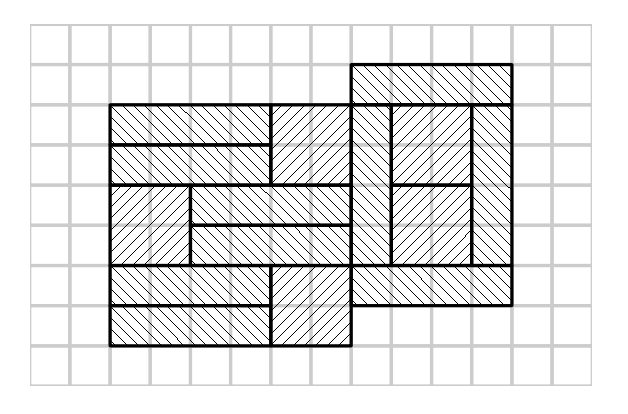
\includegraphics[scale=0.5]{tiles}

	      Lösung:
	      \begin{enumerate}
		      \item
	      \end{enumerate}
\end{enumerate}
\end{document}